\section{Performance \& Results}
\label{results}

To demonstrate the three variant WORG methods, an unconstrainted once 
through fuel cycle is modeled with the Cyclus simulator 
\cite{DBLP:journals/corr/HuffGCFMOSSW15}. In such a scenario, uranium
mining, enrichment, fuel fabrication, and storage all have effectively 
infinite capacities. The only meaningful constraints on the system are
how many light-water reactors (LWR) are built.

The base simulation begins with 100 reactors in 2016 that each produce
1 GWe, have an 18 month batch legnth with a one month reload time.
The initial fleet of LWRs retires evenly over the 40 years from 2016 to 
2056. All new reactors have 60 year life times.  The simulation itself 
follows 20 years from 2016 to 2035. This is the maximum \emph{in situ} time 
horizons expected, which may be 1, 5, 10, or 20 years.

The study here compares how WORG performs for 0\% (steady state), 1\%, 
and 2\% growth curves from an initial 90 GWe target. These are examined
using the three estimation variants.  Calling $r$ the growth rate as a 
fraction, the demand curve is thus,
\begin{equation}
\label{f-rate}
f(t) = 90 (1 + r)^t
\end{equation}
Moreover, the upper bound for the number of deployable facilities at 
each time is set to be the ceiling of ten times the total growth. 
That is, assuming ten facilities at most could be deployed in the first
year, increase the upper bound along with the growth rate.  This yields
the following expression for $N$.
\begin{equation}
\label{n-rate}
N(t) = \left\lceil 10 (1 + r)^t\right\rceil
\end{equation}
The lower bound for the number of deployed reactor is simply set to the 
zero vector, $M = \mathbf{0}$.  A maximum of 20 simulations are allowed.
This is because an \emph{in situ} method cannot afford many optimization 
iterations. The random seed for all optimizations was 424242.

Note that because of the integral nature of facility deployment, 
exactly matching a continous demand curve is not possible. Slight over- 
and under-prediction are expected for most points in time. Furthermore, 
it is unlikely that the initial facilities will match the demand curve 
themselves. If the intiial facilites do no meet the demand on their own, 
then the optimized deployment schedule is capable making up the difference.
However if the initial facilities produce more than the demand curve, 
the the optimizer is only capable of deploying zero facilities at relevant
times. This method does help make radical adjustments to accomodate 
problems with the initial conditions, such as when 50 GWe are demanded 
but 100 GWe are already being produced.

To begin the comparison, Figures \ref{demand-product-stochastic} - 
\ref{demand-product-all} display the
power production for the best-guess deployment schedule $G_1$ (solid lines),
production for the second best schedule $G_2$ (dotted lines), 
and demand curves (dashed) for 0\%, 1\%, and 2\% growth. 
Each figure shows a different estimation mechanism.

\begin{figure}[htb]
\centering
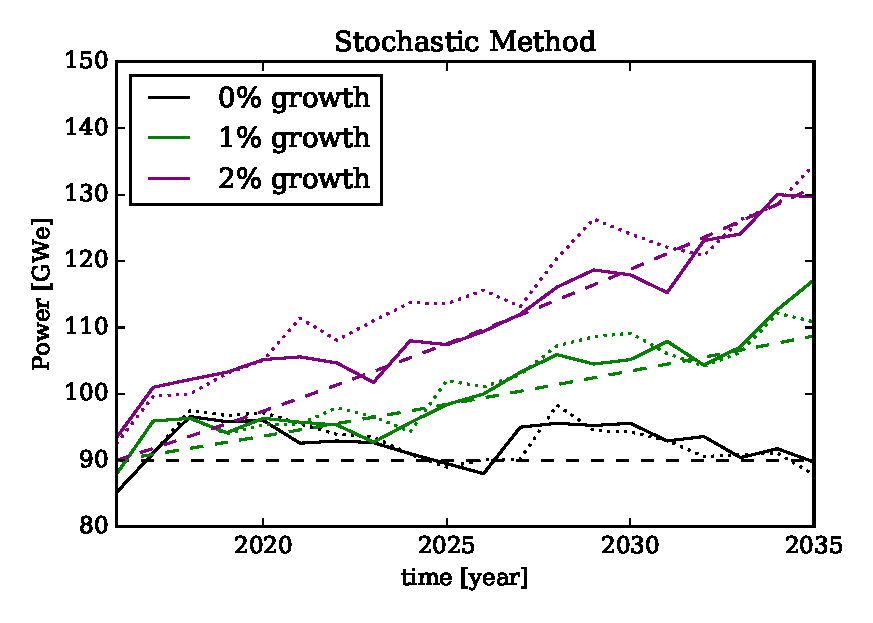
\includegraphics[width=0.9\textwidth]{demand-product-stochastic.eps}
\caption{Power production to demand comparison for 20 year deployment 
schedule optimization using only the \stochastic estimation method.
0\%, 1\%, and 2\% growth rates starting at 90 GWe are shown. Solid lines 
represent the bestguess deployment schedule.  Dotted lines are represent 
the second best guess deployment schedule. Dashed lines represent the 
demand curve that is targeted.
}
\label{demand-product-stochastic}
\end{figure}

\begin{figure}[htb]
\centering
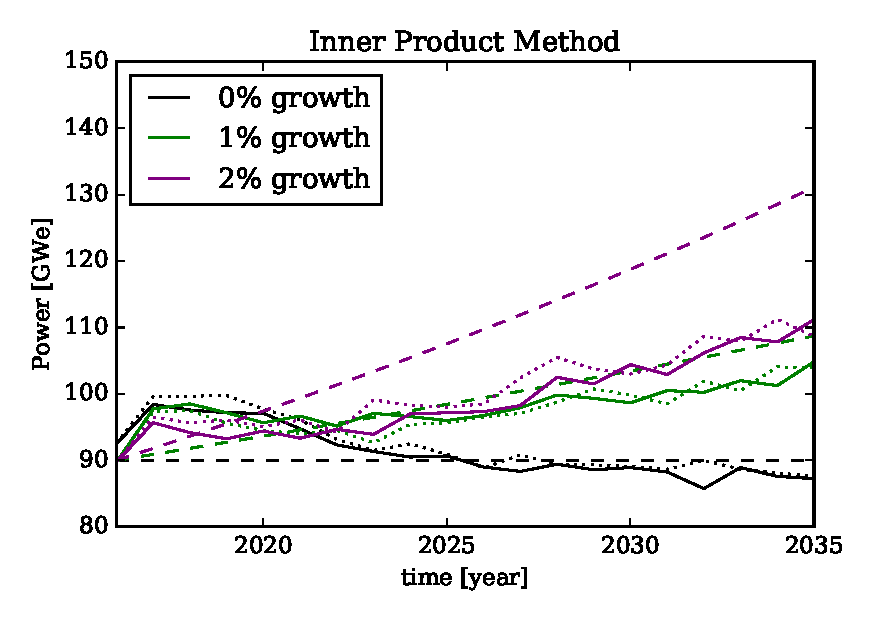
\includegraphics[width=0.9\textwidth]{demand-product-inner-product.eps}
\caption{Power production to demand comparison for 20 year deployment 
schedule optimization using only the \innerprod estimation method.
0\%, 1\%, and 2\% growth rates starting at 90 GWe are shown. Solid lines 
represent the bestguess deployment schedule.  Dotted lines are represent 
the second best guess deployment schedule. Dashed lines represent the 
demand curve that is targeted.
}
\label{demand-product-inner-product}
\end{figure}

\begin{figure}[htb]
\centering
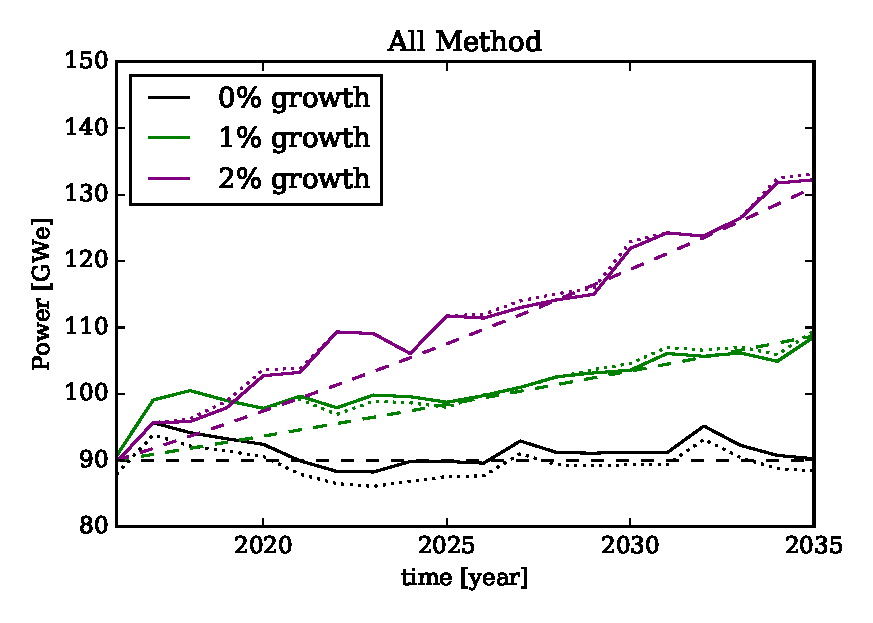
\includegraphics[width=0.9\textwidth]{demand-product-all.eps}
\caption{Power production to demand comparison for 20 year deployment 
schedule optimization using the \allflag estimation method that selects the 
best of both \stochastic and \innerprod estimations.
0\%, 1\%, and 2\% growth rates starting at 90 GWe are shown. Solid lines 
represent the bestguess deployment schedule.  Dotted lines are represent 
the second best guess deployment schedule. Dashed lines represent the 
demand curve that is targeted.}
\label{demand-product-all}
\end{figure}

As seen in Figure \ref{demand-product-stochastic}, the \stochastic only 
estimations follow the trend line of the growth curve.  However, for only 
a few regions such as for 2\% growth between 2025 - 2030, does the 
production closely match the the demand.  The second best guess for the 
deployment schedule shows a relatively large degree of excentricity. This 
indicates that $G_2$ at the end of the optimization is there to show the 
Gaussian process model regions in the $\Theta$ option space that do not work. 

Alternatively the inner product search estimation can be seen in Figure 
\ref{demand-product-inner-product}. This method does a reasonable job of
predicting a steady state scenario at later times. However, the 1\% and 2\%
curves are largely under-predicted.  For the 2\% case, this is so severe
as to be considered wholly wrong. This situation arises because the 
\innerprod method can enter into deterministic traps where the same cycle
of deployment schedules is predicted for ever.  If this happens when the 
production curve is far from an optimum, the inner product method does not
yeild a sufficient guess of the deployment schedule.

However, combining the stochastic and inner product estimation methods limits
the weakness of each method. Figure \ref{demand-product-all} shows the 
production and demand information for the \allflag estimation. By inspection, 
this method produces production curves that match the demand much more 
closely. This is especially true for later times. Over-prediction 
discrepencies for early times come from the fact the initially deployed 
facilities (100 LWRs with 18 month cycles) does not precisely match an 
initial 90 GWe target. The problem was specified this way in order to show 
that resonable deployments are still selected even in slightly 
unreasonable sitations.

